\documentclass[10pt]{article}
\usepackage[letterpaper,margin=1in]{geometry}
\usepackage{amsmath,booktabs,graphicx,array,caption,float}
\usepackage[hidelinks]{hyperref}
\usepackage{enumitem,adjustbox}
\captionsetup{font=small}
\setlist{itemsep=1pt,topsep=3pt}
% ---- numbers from the analysis scripts (was numbers.tex) ----
\newcommand{\NIspD}{320.8}
\newcommand{\NIspP}{303.5}
\newcommand{\NIspIdeal}{341.5}
\newcommand{\NetaI}{0.9417}
\newcommand{\NetaP}{0.8908}
\newcommand{\NOMEideal}{334.6}
\newcommand{\NRfourideal}{348.0}
\newcommand{\NEPS}{108}
\newcommand{\NDt}{140.2}
\newcommand{\NDe}{1.457}
\newcommand{\Nmdot}{7.9434}
\newcommand{\Ntb}{2{,}644}
\newcommand{\NLavail}{2.642}
\newcommand{\NLeng}{2.636}
\newcommand{\Netadiv}{0.9885}
\newcommand{\NthN}{37}
\newcommand{\NthE}{8}
\newcommand{\NconeEta}{0.98397}
\newcommand{\NconeTh}{0.98296}
\newcommand{\NwedgeEta}{0.98882}
\newcommand{\NwedgeTh}{0.98862}
\newcommand{\NmocMerr}{0.11}
\newcommand{\NBZpct}{12.5}
\newcommand{\NBZOF}{0.6}
\newcommand{\NBZTc}{1{,}541}
\newcommand{\NBZloss}{0.78}
\newcommand{\NOFcore}{1.92}
\newcommand{\Nliner}{83}
\newcommand{\NlinerMass}{66}
\newcommand{\Nchar}{51}
\newcommand{\Ntdesign}{3{,}305}
\newcommand{\Nepsatt}{6}
\newcommand{\NTmaxExt}{1{,}389}
\newcommand{\NTthroat}{1{,}806}
\newcommand{\NTback}{354}
\newcommand{\NTinj}{399}
\newcommand{\NdTinjZero}{152}
\newcommand{\Npu}{1.28}
\newcommand{\NMEOP}{1.47}
\newcommand{\Npreg}{1.33}
\newcommand{\Npend}{2.33}
\newcommand{\NmHe}{87}
\newcommand{\NmHeIso}{44}
\newcommand{\NmHeAdi}{73}
\newcommand{\NVbot}{460}
\newcommand{\NDcopv}{0.96}
\newcommand{\Nmtot}{1{,}373}
\newcommand{\Nshare}{21.1}
\newcommand{\Nmeng}{171}
\newcommand{\NmengH}{110}
\newcommand{\NOFopt}{2.40}
\newcommand{\NOFoptFr}{1.70}
\newcommand{\NOFeq}{1.638}
\newcommand{\NvalDb}{332.8}
\newcommand{\Nheritage}{315.1}
\newcommand{\NsweepOpt}{0.6}
\newcommand{\NhgT}{2{,}286}
\newcommand{\NqBZ}{3.1}
\newcommand{\NLcav}{59}
\newcommand{\NdPf}{26}
\newcommand{\NdPo}{20}
\newcommand{\Nstack}{5.37}
\newcommand{\Nspare}{0.63}
\newcommand{\NPe}{430}
\newcommand{\NCFvac}{1.879}
\newcommand{\NPeRatio}{0.42}
\newcommand{\NbestFrac}{70}
\newcommand{\NvacGain}{0.10}
\newcommand{\NIspMargin}{41}
\newcommand{\NDtank}{2.64}
\newcommand{\NDtankf}{2.63}
\newcommand{\Nttank}{2.2}
\newcommand{\Npbend}{6.0}
\newcommand{\NfreeO}{1.4}
\newcommand{\NfreeF}{1.6}
% ---- end numbers ----
\graphicspath{{./}{figs/}{images/}{figures/}{Figures/}}  % images in the project root or any of these folders
\title{Project ABEONA Crew Capsule Main Engine:\\Thrust Chamber, Feed System, and Pressurization Design}
\author{[Your Name]}
\date{October 2026}
\begin{document}
\maketitle

\section{Introduction}
This analysis designed the single 25~kN main engine of the Project ABEONA Crew Capsule service module and its
propellant feed and pressurization system. The engine burns nitrogen tetroxide (NTO) and monomethylhydrazine (MMH),
is pressure-fed by regulated helium, and operates only in vacuum. The work covered the inputs, the cycle and
operating-point trades, the thrust chamber, the vacuum nozzle, the thermal design, the injector, the tanks and
pressurization, the materials, and consistency checks.

All vehicle numbers were taken directly from the Crew Capsule tab of \texttt{Mission\_Breakdown.xlsx} [12]. The
Preliminary Design Report (PDR) was used for the propellant choice, architecture and packaging envelope [12]. The method
and reporting style follow the Stage 2/3 hydrolox engine report [13] and Huzel and Huang [1]. Every number in this
report was produced by the Python analysis scripts.

NASA CEA could not be installed in the analysis environment. Combustion performance was computed with an equilibrium
solver written with the CEA method (NASA RP-1311 [2]) and the NASA thermodynamic database that ships with CEA [11]. It
matched CEA output within 0.02~\% (Table~\ref{tab:valid}). Liquid MMH and NTO properties came from the RocketProps
library [6].

\section{Requirements and Inputs}
The spreadsheet values used in the design are listed in Table~\ref{tab:req}; they were used as given. The mass flow and
burn time in the sheet correspond to the minimum 280~s $I_{sp}$; the designed engine has a higher $I_{sp}$, so at the same
25~kN it uses less propellant per second and fires longer (Sec.~\ref{sec:checks}).

\begin{table}[H]\centering\small\caption{Crew Capsule requirements (spreadsheet).}\label{tab:req}\adjustbox{max width=\linewidth}{
\begin{tabular}{ll}
\toprule
Parameter & Spreadsheet value \\
\midrule
Initial / propellant / structural / payload mass, kg & 38{,}000 / 21{,}000 / 6{,}500 / 10{,}500 \\
Burnout mass, kg; mass ratio & 17{,}000; 2.235294 \\
$\epsilon$ / $\lambda$ & 0.236364 / 0.381818 \\
Required $I_{sp}$, s; $u_{eq}$, m/s & 280; 2{,}746.8 \\
$\Delta u$, m/s & 2{,}209.45 \\
Mass flow, kg/s; burn time, s & 9.1015; 2{,}307.3 \\
Thrust, engines & 25 kN, 1 \\
$T/W$ Earth, initial / burnout & 0.0671 / 0.1499 \\
$T/W$ Moon, initial / burnout & 0.405 / 0.905 \\
MMH / NTO density, kg/m$^3$ & 875 / 1{,}440 \\
\bottomrule
\end{tabular}
}\end{table}

Differences between the spreadsheet and the PDR are listed in Table~\ref{tab:audit}; the spreadsheet value was carried
in every case. The PDR tanks (2.6~m spheres, 9.203~m$^3$) leave only \NfreeO~\% (NTO) and \NfreeF~\% (MMH) free volume
for the spreadsheet propellant load, which is not enough for ullage gas or a propellant management device, so the
tanks were resized (Sec.~\ref{sec:tanks}).

\begin{table}[H]\centering\small\caption{Inputs audit: spreadsheet versus PDR.}\label{tab:audit}\adjustbox{max width=\linewidth}{
\begin{tabular}{p{4.0cm}p{3.0cm}p{3.0cm}p{5.0cm}}
\toprule
Item & Spreadsheet & PDR & Disposition \\
\midrule
Payload ratio $\lambda$ & 0.3818 & 0.304 & Spreadsheet carried \\
$\Delta u$, m/s & 2{,}209.5 & 2{,}200 & Spreadsheet carried \\
Mixture ratio & not given & 1.65 (AJ10) & PDR value used \\
Launch Escape System & Stage 3 payload 45,000 kg & 7,000 kg (Fig. 9) & Outside the 38,000 kg capsule mass \\
Propellant volume, m$^3$ & NTO 9.080, MMH 9.057 & 9.203 each & Only 1.4 / 1.6 \% free; tanks resized \\
Aft envelope & -- & 2.01 m base to exit; 0.5 m cone & Engine length is the limit \\
\bottomrule
\end{tabular}
}\end{table}

\section{Design Decisions and Assumptions}
\begin{table}[H]\centering\small\caption{Approved design decisions.}\label{tab:dec}
\begin{tabular}{lp{11.5cm}}\toprule Item & Decision \\\midrule
Propellants & NTO / MMH \\
Cycle & Pressure-fed, regulated helium \\
Chamber pressure & 0.862~MPa (125 psia), nozzle-entrance stagnation pressure (AJ10-190 heritage) \\
Mixture ratio & 1.65 overall (PDR) \\
Nozzle & Rao optimum-thrust bell for vacuum, 80~\% length, area ratio set by the engine-length envelope \\
Cooling & Ablative silica-phenolic chamber and throat; fuel-rich outer injector ring; C-103 nozzle extension \\
Pressurization & Helium in composite bottles, two series regulators, check valves, relief valve \\
Propellant acquisition & Screen-channel propellant management device (PMD) in each tank \\
\bottomrule\end{tabular}\end{table}

Main assumptions:
\begin{enumerate}
\item Steady state; combustion products are ideal gases in chemical equilibrium; $g = 9.81$~m/s$^2$ as in the spreadsheet.
\item Delivered efficiency calibrated to the AJ10-190 Orbital Maneuvering Engine (OME): 315.1~s at 0.862~MPa, area ratio 55,
O/F 1.65 [15,16]. Its ideal value is \NOMEideal~s, so $\eta_{I_{sp}} = $~\NetaI. The pessimistic case uses the R-4D-11
(310~s against \NRfourideal~s ideal, $\eta_{I_{sp}} = $~\NetaP) [15]. $\eta_{c^*} = 0.99$ [16].
\item Propellants at 293~K; tank volumes use the spreadsheet densities.
\item Gas-side heat transfer by Bartz [9] with no hypergolic calibration; a 1.3 factor was used to size the wall protection.
\item Ablator properties, material limits, component pressure drops and some component masses are assumed values, to be
verified.
\end{enumerate}

\section{Cycle and Operating-Point Selection}\label{sec:trade}
\subsection{Envelope}
In PDR Fig.~9 the service-module section is 6~m long and 4.98~m in diameter. The 2.01~m dimension runs from the
service-module base to the nozzle exit, and the 0.5~m dimension is the aft-cone height. The resized tanks leave \Nspare~m
free in the 6~m section below the NTO tank, so the engine (gimbal plane to nozzle exit) may be \NLavail~m long. The
length, not the 2.0~m drawn exit diameter, limited the nozzle at every chamber pressure studied.

\subsection{Cycle}
Five feed cycles were sized with the same mass models (Table~\ref{tab:cycle}). A blowdown system needs 50~\% more tank
volume and its thrust falls 3:1 as the tanks empty. Regulating first and blowing down at the end saves only a few
kilograms of helium. Pump-fed engines reach higher pressure and area ratio, but the gas-generator figures come from an
uprated OME that never flew [16] and the electric pump needs a large battery. The pressure-fed regulated cycle was
selected: it is the AJ10-190 / European Service Module arrangement, it has no rotating machinery, and it restarts simply.

\begin{table}[H]\centering\small\caption{Cycle trade (nominal efficiency).}\label{tab:cycle}\adjustbox{max width=\linewidth}{
\begin{tabular}{lrrrrl}
\toprule
Cycle & $P_c$, MPa & $\varepsilon$ & $I_{sp}$, s & System mass, kg & Remark \\
\midrule
Pressure-fed, regulated He & 0.86 & 106 & 321.7 & 1{,}121 & heritage AJ10-190 / ESM \\
Pressure-fed, blowdown 3:1 & 2.59 & 106 & 321.7 & 2{,}937 & tank volume 27.3 m3 (x1.50), thrust 75 -> 25 kN \\
Regulated then blowdown (last 15 %) & 0.86 & 106 & 321.4 & 1{,}116 & saves ~5 kg He \\
Electric pump-fed & 2.50 & 295 & 329.9 & 1{,}000 & 45 kW, battery 357 kg, pumps 50 kg \\
Gas-generator pump-fed & 2.41 & 285 & 326.4 & 663 & UOME (never flown) \\
\bottomrule
\end{tabular}
}\end{table}

\subsection{Chamber pressure}
Raising the chamber pressure shrinks the throat, so a larger area ratio fits the same length and $I_{sp}$ rises.
However the tanks must run at about twice the chamber pressure, so tank, helium and bottle mass grow quickly
(Table~\ref{tab:pc}, Fig.~\ref{fig:pc}). The lightest system is near \NsweepOpt~MPa. The OME value of 0.862~MPa was
selected because the efficiency calibration applies there directly and the system is still light.

\begin{table}[H]\centering\small\caption{Pressure-fed chamber-pressure sweep.}\label{tab:pc}\adjustbox{max width=\linewidth}{
\begin{tabular}{rrrrrrrrr}
\toprule
$P_c$, MPa & $\varepsilon$ & $D_e$, m & $I_{sp}$, s & $p_{tank}$, MPa & Tanks, kg & He, kg & Bottles, kg & Engine, kg \\
\midrule
0.600 & 75.4 & 1.484 & 318.3 & 1.20 & 443 & 41 & 192 & 143 \\
0.862 & 106.2 & 1.462 & 321.7 & 1.72 & 637 & 60 & 281 & 143 \\
1.000 & 122.3 & 1.455 & 323.0 & 2.00 & 739 & 71 & 330 & 143 \\
1.250 & 151.3 & 1.444 & 324.8 & 2.50 & 923 & 90 & 420 & 142 \\
1.500 & 180.2 & 1.436 & 326.2 & 3.00 & 1{,}108 & 110 & 515 & 142 \\
2.000 & 237.9 & 1.426 & 328.3 & 4.00 & 1{,}477 & 153 & 717 & 142 \\
2.500 & 295.4 & 1.418 & 329.9 & 5.00 & 1{,}847 & 200 & 936 & 141 \\
\bottomrule
\end{tabular}
}\end{table}
\begin{figure}[H]\centering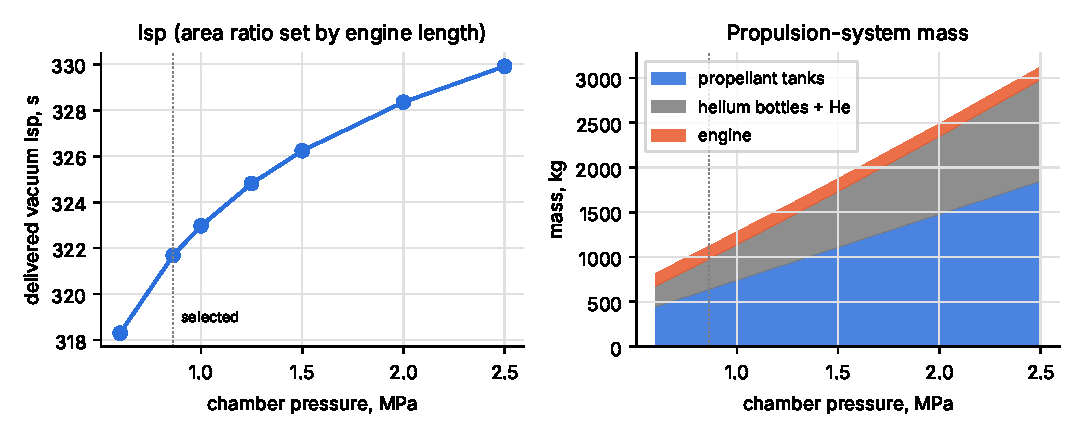
\includegraphics[width=0.95\textwidth]{fig_pc_trade.pdf}
\caption{Chamber-pressure trade.}\label{fig:pc}\end{figure}

\subsection{Mixture ratio}
The ideal $I_{sp}$ peaks at O/F \NOFopt{} with shifting equilibrium and \NOFoptFr{} with frozen chemistry (Fig.~\ref{fig:of});
a real engine of this size peaks between the two, near 1.9 [5]. The equal-volume O/F with the spreadsheet densities is
1.646, which is why the PDR tanks are equal. O/F 1.65 was kept. The core of the injector runs at O/F \NOFcore{}
anyway because the outer ring is fuel-rich (Sec.~\ref{sec:cool}).
\begin{figure}[H]\centering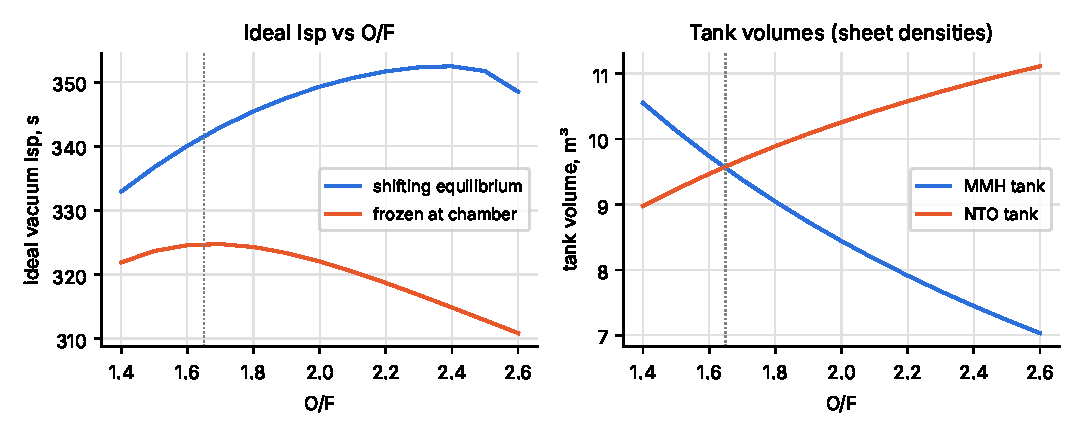
\includegraphics[width=0.95\textwidth]{fig_of_trade.pdf}
\caption{Ideal $I_{sp}$ and tank volumes versus O/F.}\label{fig:of}\end{figure}

\section{Thrust Chamber}
\subsection{Ideal performance}
Table~\ref{tab:ideal} gives the ideal vacuum performance at 0.862~MPa, O/F 1.65 and area ratio \NEPS. Reactant heats of
formation were the CEA input-card values (NTO $-19.56$~kJ/mol, MMH $+53.97$~kJ/mol); the database values give
\NvalDb~s instead of 332.4~s at the validation point. A closed-form one-dimensional nozzle with the chamber $\gamma$
reproduced the frozen $c^*$ within 0.07~\%.
\begin{table}[H]\centering\small\caption{Ideal vacuum performance.}\label{tab:ideal}\adjustbox{max width=\linewidth}{
\begin{tabular}{lrrr}
\toprule
Quantity & Shifting & Frozen & Closed form, diff. vs frozen \\
\midrule
$T_c$, K & 3{,}042.3 & 3{,}042.3 & -- \\
$c^*$, m/s & 1{,}737.9 & 1{,}698.6 & 1{,}699.7 (+0.07 \%) \\
$C_{F,vac}$ & 1.9276 & 1.8753 & 1.9143 (+2.08 \%) \\
$I_{sp,vac}$, s & 341.5 & 324.7 & 331.7 (+2.15 \%) \\
Exit pressure, Pa & 430 & 331 & -- \\
\bottomrule
\end{tabular}
}\end{table}
\begin{table}[H]\centering\small\caption{Solver validation against NASA CEA.}\label{tab:valid}\adjustbox{max width=\linewidth}{
\begin{tabular}{lrrr}
\toprule
Quantity & NASA CEA & This solver & Diff., \% \\
\midrule
$T_c$, K & 3{,}466.8 & 3{,}466.8 & -0.001 \\
$c^*$ shifting, m/s & 2{,}350.6 & 2{,}350.6 & +0.001 \\
$C_F$ shifting & 1.9739 & 1.9738 & -0.006 \\
$I_{sp}$ shifting, s & 473.1 & 473.1 & +0.002 \\
$c^*$ frozen, m/s & 2{,}319.6 & 2{,}319.6 & -0.002 \\
$C_F$ frozen & 1.9329 & 1.9328 & -0.006 \\
$I_{sp}$ frozen, s & 457.2 & 457.2 & -0.008 \\
NTO/MMH, O/F 1.0--2.9: largest difference & -- & -- & $I_{sp}$ 0.02, $c^*$ 0.00, $T_c$ 0.00 \\
\bottomrule
\end{tabular}
}\end{table}

\subsection{Delivered performance and geometry}
The model reproduces the OME flight value at its own area ratio (\Nheritage~s against 315.1~s). The delivered vacuum
$I_{sp}$ of this engine is \NIspD~s (\NIspP~s pessimistic), \NIspMargin~s above the 280~s requirement. The geometry is
in Table~\ref{tab:geom}.
\begin{table}[H]\centering\small\caption{Thrust-chamber geometry and delivered performance.}\label{tab:geom}\adjustbox{max width=\linewidth}{
\begin{tabular}{lll}
\toprule
Parameter & Value & Basis \\
\midrule
Mass flow (NTO / MMH), kg/s & 7.9434 (4.9459 / 2.9975) & $F/(I_{sp}g)$ \\
Delivered vacuum $I_{sp}$ (pessimistic), s & 320.8 (303.5) & AJ10-190 (R-4D-11) calibration \\
Delivered $c^*$, $C_{F,vac}$ & 1{,}675.1 m/s, 1.8789 & $\eta_{c^*}$ 0.99 \\
Throat area / diameter & 154.36 cm$^2$ / 140.2 mm & $\dot m c^*/P_c$ \\
Area ratio / exit diameter & 108 / 1.457 m & engine-length limit \\
Contraction ratio / chamber diameter & 3.0 / 242.8 mm & H\&H practice (assumed) \\
$L^*$ / chamber volume & 0.80 m / 12.35 L & H\&H Table 4-1 (assumed) \\
Cylinder / convergent length & 182 / 136 mm & 30$^\circ$ cone, $R_1 = 1.5 r_t$ \\
Injector-end pressure & 0.8827 MPa (1.0241 $P_c$) & Rayleigh \\
Injector face to throat / throat to exit & 0.318 / 1.968 m & 80 \% bell \\
Engine length incl. 0.35 m head & 2.636 m & available 2.642 m \\
\bottomrule
\end{tabular}
}\end{table}

\section{Vacuum Nozzle}
\subsection{Contour}
The contour was designed with an axisymmetric method-of-characteristics (MOC) solver. Along the characteristics
\begin{equation}
d(\theta \pm \nu) = \pm\frac{\sin\theta\sin\mu}{y}\,ds,
\end{equation}
(upper sign on C$^-$) [7,8]. The wall is a $0.382r_t$ arc from the throat to $\theta_N$ followed by a smooth curve to the
exit lip at angle $\theta_E$. $\theta_N$ and $\theta_E$ were searched for maximum thrust at fixed length and exit
diameter, which is Rao's optimum-thrust problem [10]. The solver was checked against a 15$^\circ$ cone
(\NconeEta{} against $(1+\cos\alpha)/2 = $~\NconeTh) and a flat wedge (\NwedgeEta{} against $\sin\alpha/\alpha = $~\NwedgeTh),
with \NmocMerr~\% mass-flow error. Results are in Table~\ref{tab:noz} and Fig.~\ref{fig:contour}.

\begin{table}[H]\centering\small\caption{Rao vacuum bells at area ratio \NEPS{} (MOC).}\label{tab:noz}\adjustbox{max width=\linewidth}{
\begin{tabular}{lrrrrr}
\toprule
Length (\% of 15$^\circ$ cone) & 70 & 80 & 90 & 100 & cone \\
\midrule
Length, m & 1.722 & \textbf{1.968} & 2.214 & 2.461 & 2.461 \\
$\theta_N$, deg & 39.0 & \textbf{37.0} & 34.0 & 34.0 & 15.0 \\
$\theta_E$, deg & 9.0 & \textbf{8.0} & 7.0 & 4.0 & 15.0 \\
Divergence efficiency & 0.98225 & \textbf{0.98854} & 0.99201 & 0.99414 & 0.98397 \\
\bottomrule
\end{tabular}
}\end{table}
\begin{figure}[H]\centering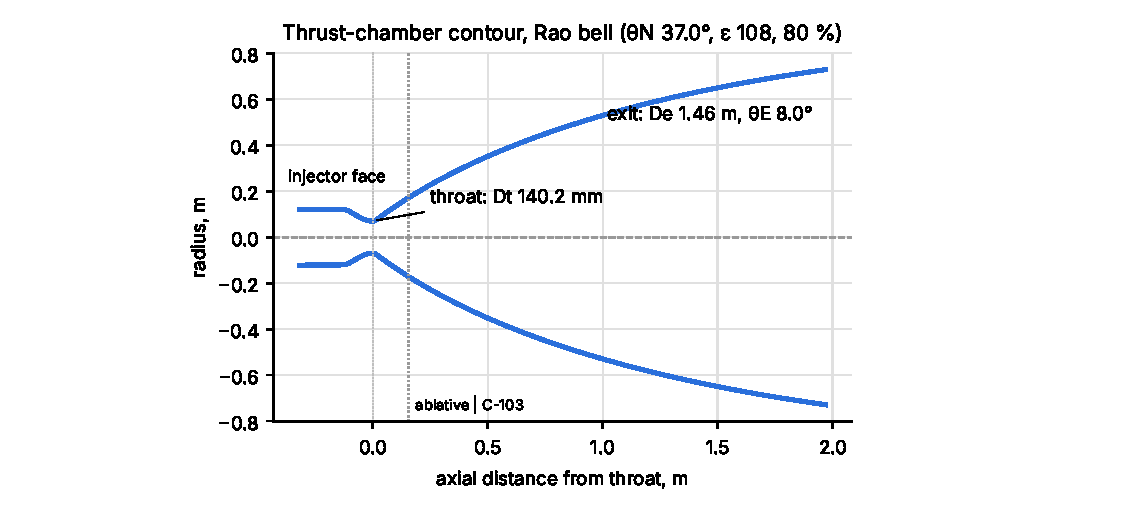
\includegraphics[width=0.95\textwidth]{fig_contour.pdf}
\caption{Thrust-chamber contour from the injector face to the nozzle exit.}\label{fig:contour}\end{figure}

\subsection{Vacuum-optimization check}
The engine fires only in space, so it was checked three ways that the nozzle is optimized for vacuum:
\begin{enumerate}
\item The MOC thrust integral uses zero outside pressure, so the bell maximizes vacuum thrust.
\item The exit pressure is only \NPe~Pa (\NPeRatio~\% of sea-level pressure), with a vacuum thrust coefficient of \NCFvac.
At sea level the flow would separate inside the bell, so this is a vacuum-only nozzle, as intended.
\item The length is fixed by the service module, so a shorter bell allows a larger area ratio. Table~\ref{tab:vac} and
Fig.~\ref{fig:vac} show the delivered vacuum $I_{sp}$ for each bell length at the same overall engine length. The best is
the \NbestFrac~\% bell, \NvacGain~s above the selected 80~\% bell, which is within the accuracy of the method. The 80~\% bell was kept.
\end{enumerate}
\begin{table}[H]\centering\small\caption{Vacuum $I_{sp}$ at the same engine length.}\label{tab:vac}\adjustbox{max width=\linewidth}{
\begin{tabular}{rrrrr}
\toprule
Bell length, \% & Area ratio & Exit diameter, m & Divergence eff. & Vacuum $I_{sp}$, s \\
\midrule
70 & 139 & 1.650 & 0.9823 & 320.97 \\
80 & 109 & 1.461 & 0.9885 & \textbf{320.88} \\
90 & 87 & 1.314 & 0.9920 & 319.98 \\
100 & 72 & 1.197 & 0.9941 & 318.76 \\
\bottomrule
\end{tabular}
}\end{table}
\begin{figure}[H]\centering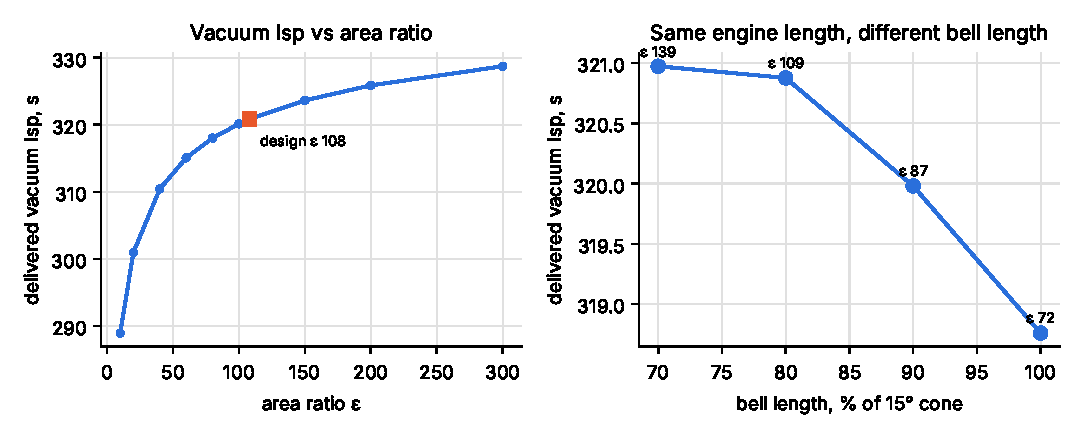
\includegraphics[width=0.95\textwidth]{fig_vacuum.pdf}
\caption{Left: delivered vacuum $I_{sp}$ against area ratio. Right: bell length at fixed engine length.}\label{fig:vac}\end{figure}

\section{Thermal Design}\label{sec:cool}
\subsection{Heat flux}
The gas-side heat transfer coefficient followed Bartz [9; 1, Eq.~4-13]:
\begin{equation}
h_g = C\frac{0.026}{D_t^{0.2}}\left(\frac{\mu^{0.2}c_p}{Pr^{0.6}}\right)_0\left(\frac{P_c}{c^*}\right)^{0.8}
\left(\frac{D_t}{R_c}\right)^{0.1}\left(\frac{A_t}{A}\right)^{0.9}\sigma .
\end{equation}
At the throat $h_g$ is \NhgT~W/(m$^2$K). The heat flux along the engine is plotted in Fig.~\ref{fig:q}; it peaks at
the throat at \NqBZ~MW/m$^2$ into a 700~K wall.

\subsection{Fuel-rich outer ring}
The combustion gas is about 3,000~K, well above what any ablative can survive for the \Ntb~s of total firing. The
injector's outer ring of elements was therefore run fuel-rich, at O/F \NBZOF{}. This puts a layer of cooler
(\NBZTc~K), fuel-rich gas against the wall, much as the OME uses a fuel film. \NBZpct~\% of the flow goes through the
outer ring. That is the smallest amount that keeps the throat surface below the temperature at which silica phenolic
starts to wear away, even with the heat flux raised by 30~\%. It costs \NBZloss~s of $I_{sp}$, which is already
included in the delivered value. A fuel film from separate orifices was the alternative; the fuel-rich ring was chosen
because it uses the same injector elements and stays attached to the wall over the whole chamber.

\subsection{Ablative liner and nozzle extension}
\textbf{Material choice.} The chamber and throat are lined with tape-wrapped silica phenolic. The two common rocket
ablatives are silica phenolic and carbon phenolic. Carbon phenolic handles higher temperatures, but its carbon reacts
with the water vapor and carbon dioxide in NTO/MMH exhaust and wears away, and it conducts heat well, so it needs a
thicker insulating layer behind it. Silica phenolic forms a glassy surface that holds up in this exhaust, insulates
well, and is the material used on the Apollo service-module engine and the Delta second-stage AJ10 engines. Silica
phenolic was chosen.

\textbf{How it works.} As the liner heats, the resin near the hot surface turns to char, which insulates the material
behind it. The liner wears away only if its surface passes about 1,900~K. The fuel-rich ring keeps the hottest point,
the throat, at \NTthroat~K, so the throat does not grow during the mission.

\textbf{Results.} The liner runs from the injector face to area ratio \Nepsatt{}. It was sized for \Ntdesign~s of
firing, 25~\% more than the total firing time. The char reaches \Nchar~mm deep, and the liner is \Nliner~mm thick
(\NlinerMass~kg) so that the outer titanium case stays below 420~K; it ends at \NTback~K (Fig.~\ref{fig:char}). Beyond
area ratio \Nepsatt{} the gas is cool enough for a thin C-103 niobium skirt with a silicide coating, as on the Apollo
service-module engine; it peaks at \NTmaxExt~K, under its 1,600~K limit (Fig.~\ref{fig:wall}). After the longest firing,
heat stored in the liner flows back into the injector; an insulating ring between the two keeps the injector near
\NTinj~K, below the 442~K boiling point of MMH in the manifold. Without it the injector would rise about \NdTinjZero~K.

\begin{table}[H]\centering\small\caption{Thermal design results.}\label{tab:cool}\adjustbox{max width=\linewidth}{
\begin{tabular}{ll}
\toprule
Item & Value \\
\midrule
Liner material & silica phenolic (tape wrapped) \\
Liner covers & injector face to area ratio 6 (0.474 m long) \\
Fuel-rich outer ring & 12.5 \% of the flow at O/F 0.6 (1{,}541 K gas) \\
Hottest liner surface (throat) & 1{,}806 K (wear starts at 1{,}900 K) \\
Liner thickness / mass & 82.6 mm / 66.4 kg \\
Charred depth at end of firing & 50.9 mm (design life 3{,}305 s) \\
Outer case temperature at end of firing & 354 K (limit 420 K) \\
Surface wear (recession) & 1.38 mm max., none at the throat \\
Nozzle extension & C-103 from area ratio 6, max. 1{,}389 K \\
Injector after a long firing & about 399 K with insulating ring \\
\bottomrule
\end{tabular}
}\end{table}
\begin{figure}[H]\centering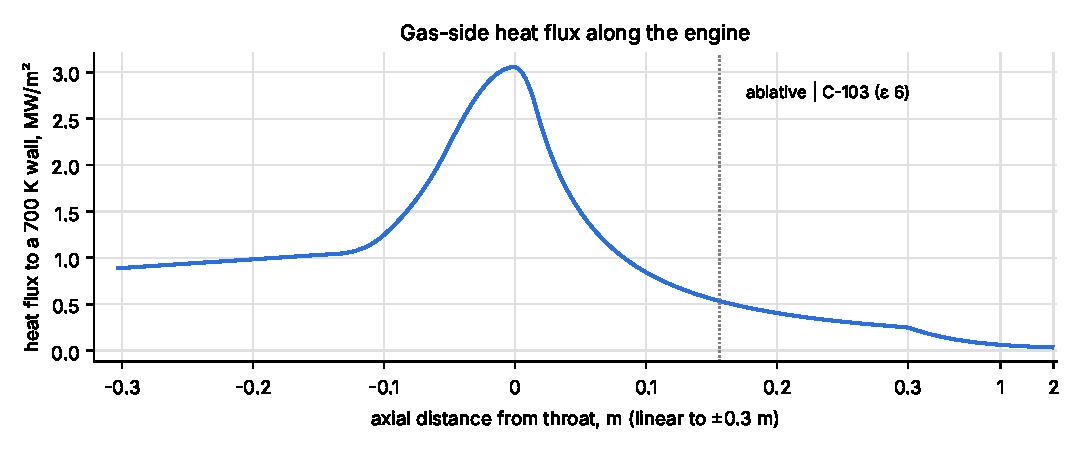
\includegraphics[width=0.92\textwidth]{fig_heatflux.pdf}
\caption{Gas-side heat flux along the engine.}\label{fig:q}\end{figure}
\begin{figure}[H]\centering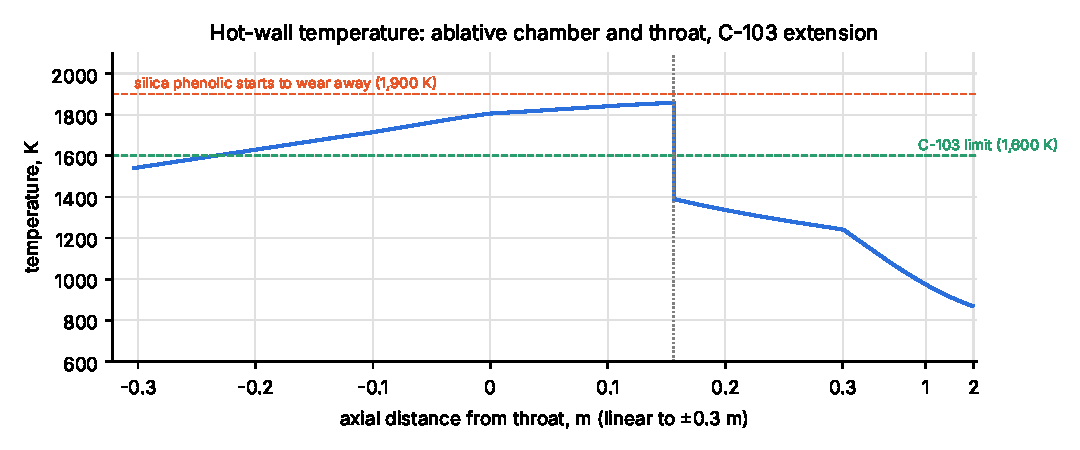
\includegraphics[width=0.92\textwidth]{fig_walltemp.pdf}
\caption{Hot-wall temperature: silica-phenolic liner (left of the dotted line) and C-103 extension.}\label{fig:wall}\end{figure}
\begin{figure}[H]\centering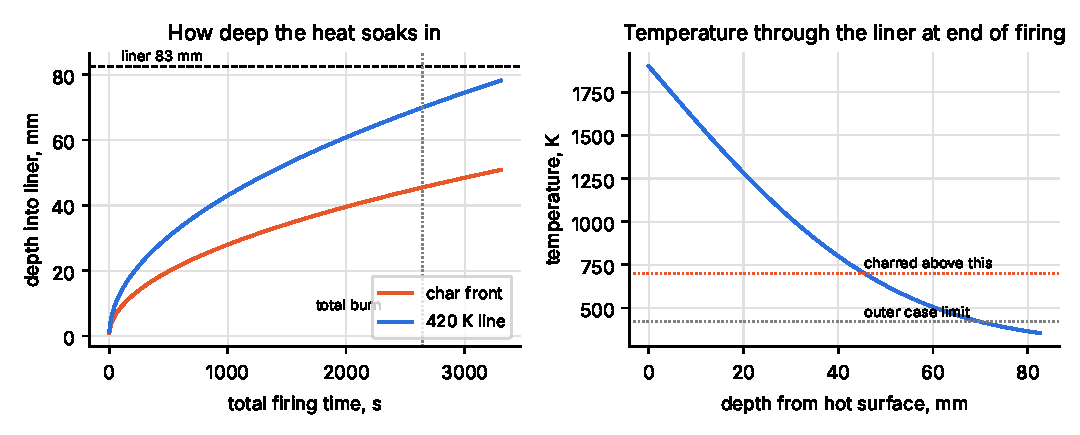
\includegraphics[width=0.92\textwidth]{fig_char.pdf}
\caption{Silica-phenolic liner at the throat.}\label{fig:char}\end{figure}

\section{Injector}
Unlike-doublet (NTO--MMH) impinging elements were used, as on the Apollo service-module engine. The NTO pressure drop is
20~\% of the injector-end pressure [1]; the MMH orifices were sized for the best mixing by Rupe's criterion
$\rho_o V_o^2 d_o = \rho_f V_f^2 d_f$, giving \NdPf~\%. Both drops exceed 15~\%, which keeps the feed system from coupling
with the combustion. Twelve quarter-wave acoustic cavities, as on the OME [16], are tuned to the first tangential mode
and are \NLcav~mm deep (Tables~\ref{tab:inj} and \ref{tab:acoustic}).
\begin{table}[H]\centering\small\caption{Injector design.}\label{tab:inj}\adjustbox{max width=\linewidth}{
\begin{tabular}{lrr}
\toprule
Parameter & Core & Outer ring \\
\midrule
Element type / count & unlike doublet / 120 & unlike doublet / 48 \\
NTO / MMH per element, g/s & 38.1 / 19.8 & 7.8 / 12.9 \\
Orifice diameter NTO / MMH, mm & 1.753 / 1.338 & 0.791 / 1.081 \\
Jet velocity NTO / MMH, m/s & 15.7 / 23.0 & 15.7 / -- \\
$\Delta P$ / injector-end pressure, NTO / MMH & 20 \% / 26 \% & shared manifolds \\
Momentum ratio, spray angle & 1.31, +4.4$^\circ$ & -- \\
\bottomrule
\end{tabular}
}\end{table}
\begin{table}[H]\centering\small\caption{Acoustic modes and cavities.}\label{tab:acoustic}\adjustbox{max width=\linewidth}{
\begin{tabular}{lr}
\toprule
Quantity & Value \\
\midrule
Chamber sound speed, m/s & 1{,}236 \\
1T / 1R / 1L frequency, Hz & 2{,}984 / 6{,}210 / 1{,}947 \\
Quarter-wave cavity depth, mm (12 cavities) & 59.4 \\
Injector mass (304L), kg & 10.0 \\
\bottomrule
\end{tabular}
}\end{table}

\section{Feed and Pressurization System}
\subsection{Pressure ladder and lines}
The pressure ladder (Fig.~\ref{fig:ladder}) starts at the chamber and adds each loss on the way back to the tank: the
injector, the engine valve, a trim orifice, a filter, the gimbal flex line, the feed line, a latch valve and the tank
outlet. Both tanks run at the same regulated pressure, \Npu~MPa; the trim orifices make up the difference between the
two sides. Lines were sized for 4~m/s or less (Table~\ref{tab:lines}); because the engine valves close in about 50~ms,
the pressure surge on shutdown stays small.
\begin{figure}[H]\centering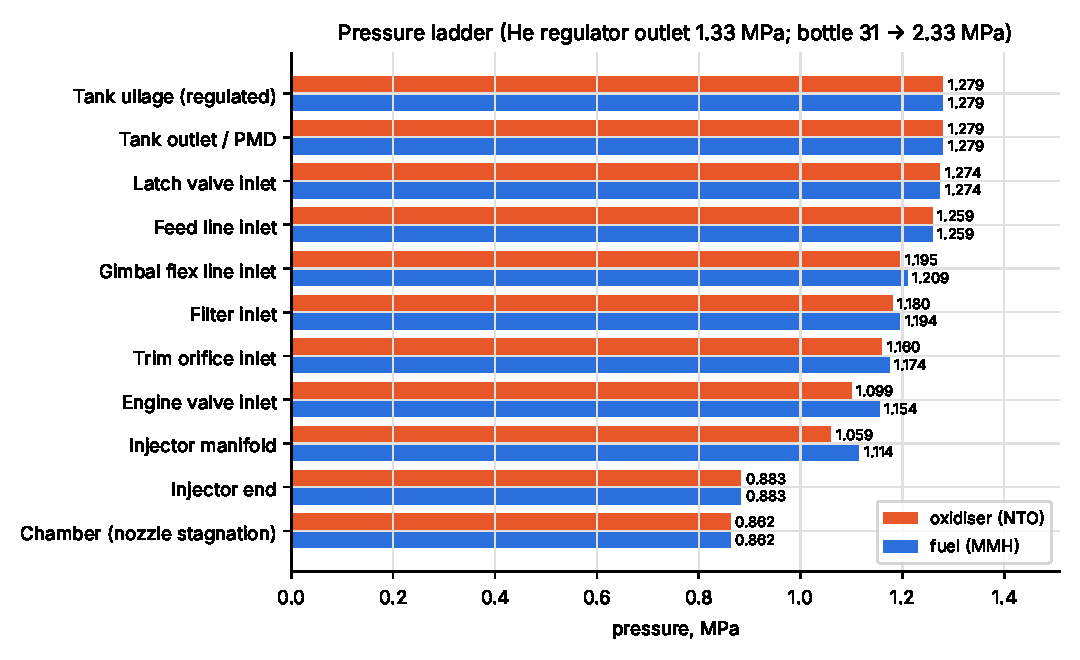
\includegraphics[width=0.9\textwidth]{fig_ladder.pdf}
\caption{Pressure ladder at the design point.}\label{fig:ladder}\end{figure}
\begin{table}[H]\centering\small\caption{Feed lines.}\label{tab:lines}\adjustbox{max width=\linewidth}{
\begin{tabular}{lrr}
\toprule
Parameter & NTO & MMH \\
\midrule
Line length (assumed), m & 2.0 & 5.5 \\
Tube OD $\times$ wall, in & 1.5 $\times$ 0.065 & 1.5 $\times$ 0.065 \\
Velocity, m/s & 3.61 & 3.60 \\
Line + fittings $\Delta P$, kPa & 63.9 & 49.6 \\
Surge at 50 ms valve closure, MPa & 0.416 & 0.693 \\
Trim orifice $\Delta P$, kPa & 60 & 20 \\
\bottomrule
\end{tabular}
}\end{table}

\subsection{Tanks}\label{sec:tanks}
Each tank holds the spreadsheet propellant mass at the spreadsheet density, plus 5~\% ullage (gas space and room for
the liquid to expand when warm) and 0.5~\% for the PMD. One titanium sphere per propellant was kept, as in the PDR:
\NDtankf~m (MMH, upper) and \NDtank~m (NTO, lower). Stacked, they are \Nstack~m tall and fit in the 6~m by 4.98~m
section. The walls are \Nttank~mm Ti-6Al-4V, sized with a burst factor of 2.0 on the \NMEOP~MPa maximum operating
pressure (Table~\ref{tab:tanks}). A screen-channel PMD in each tank holds liquid over the outlet in weightlessness, so
the engine can start without first firing thrusters to settle the propellant.
\begin{table}[H]\centering\small\caption{Propellant tanks.}\label{tab:tanks}\adjustbox{max width=\linewidth}{
\begin{tabular}{lrr}
\toprule
Parameter & MMH & NTO \\
\midrule
Propellant mass, kg & 7{,}925 & 13{,}075 \\
Propellant volume (sheet density), m$^3$ & 9.057 & 9.080 \\
Tank volume (+5 \% ullage, +0.5 \% PMD), m$^3$ & 9.555 & 9.580 \\
Sphere inner diameter, m & 2.633 & 2.635 \\
Max. operating pressure, MPa & 1.47 & 1.47 \\
Wall thickness (Ti-6Al-4V), mm & 2.16 & 2.16 \\
Shell / PMD mass, kg & 271 / 15 & 272 / 15 \\
\bottomrule
\end{tabular}
}\end{table}

\subsection{Helium pressurization}
Helium pushes the propellants out of the tanks. As each tank empties, helium fills the space the liquid leaves, so at the
end both tanks are full of helium at \Npu~MPa. That helium is stored at 31~MPa in four composite bottles and fed through
regulators that hold the tanks at a constant pressure while the bottles run down (Fig.~\ref{fig:he}). The bottles cannot be
emptied completely: the regulator needs about 1~MPa above its outlet, so the bottles stop being useful at \Npend~MPa
and the helium left in them is carried too.

How much helium is needed depends on the bottle temperature. If the bottles stay warm as they empty, \NmHeIso~kg is
enough; if the gas cools as it expands, as it does in a fast draw, it loses pressure faster and \NmHeAdi~kg is needed.
The design carries the cold-bottle amount at 273~K plus 10~\% margin, \NmHe~kg, in four \NVbot~L bottles
(\NDcopv~m diameter) that fit in the gap beside the tanks (Table~\ref{tab:he}). In this cold case the bottles still hold \Npbend~MPa when the tanks are empty, above the \Npend~MPa floor; that is the margin.
\begin{table}[H]\centering\small\caption{Helium system.}\label{tab:he}\adjustbox{max width=\linewidth}{
\begin{tabular}{ll}
\toprule
Item & Value \\
\midrule
Helium if the bottles stay warm (isothermal), kg & 43.9 \\
Helium if the bottles cool as they empty (adiabatic), kg & 73.2 \\
Carried (adiabatic at 273 K + 10 \%), kg & 86.5 \\
Bottles & 4 composite spheres, 460 L each, 0.96 m dia., 31 MPa \\
Bottle mass (all four), kg & 380 \\
Bottle pressure when the tanks are empty, MPa & 5.96 \\
\bottomrule
\end{tabular}
}\end{table}
\begin{figure}[H]\centering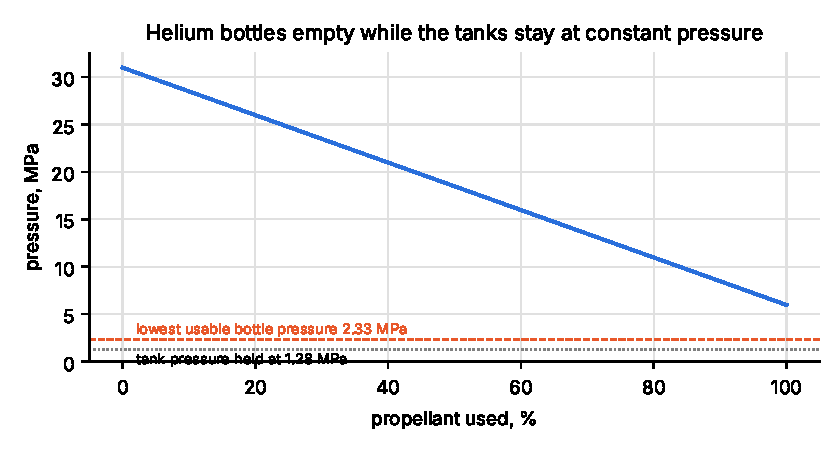
\includegraphics[width=0.62\textwidth]{fig_helium.pdf}
\caption{Helium bottle pressure as the propellant is used (design case).}\label{fig:he}\end{figure}

\section{Materials}
Table~\ref{tab:mat} compares each part's operating condition with its allowable.
\begin{itemize}
\item \textbf{Ti-6Al-4V (tanks, chamber case).} Strong and light, compatible with both propellants, and used on the
Apollo and Orion service-module tanks. Titanium can crack in NTO that contains too little nitric oxide, so the NTO must
be bought to MIL-PRF-26539 with its nitric-oxide content checked.
\item \textbf{Silica phenolic (chamber and throat liner).} Chosen in Sec.~\ref{sec:cool}: it chars into a good
insulator and does not wear away below about 1,900~K.
\item \textbf{C-103 niobium with R512E silicide coating (nozzle extension).} Keeps its strength at 1,600~K; the coating
stops oxidation. Used on the Apollo service-module and OME nozzle extensions.
\item \textbf{304L stainless (injector) and 321 stainless (lines).} Compatible with both propellants, easy to weld, and
heavy enough in the injector to soak up heat after shutdown.
\item \textbf{Composite helium bottles (titanium liner, carbon wrap).} About three times lighter than all-titanium
bottles; they hold only helium.
\item \textbf{PTFE and PCTFE (seals, valve seats).} Resist NTO, which attacks most rubbers; usable far beyond the
283--305~K propellant range.
\end{itemize}
\begin{table}[H]\centering\small\caption{Materials analysis (allowables assumed, to be verified).}\label{tab:mat}\adjustbox{max width=\linewidth}{
\begin{tabular}{p{2.6cm}p{2.6cm}p{3.6cm}p{3.3cm}p{2.2cm}}
\toprule
Part & Material & Operating condition & Allowable & Margin \\
\midrule
Propellant tanks & Ti-6Al-4V & 448 MPa at MEOP & 828 MPa yield, 895 MPa ultimate & factor 2.00 on ultimate (2.0 required) \\
Chamber/throat liner & silica phenolic & 1806 K surface & 1,900 K (wear onset) & 94 K \\
Liner back face / case & Ti-6Al-4V case & 354 K, 108 MPa & 420 K bond line, 828 MPa & 66 K; factor 7.7 \\
Nozzle extension & C-103 + R512E & 1389 K & 1,600 K & 211 K \\
Injector & 304L stainless & 399 K after shutdown & 442 K (MMH boils at 1 MPa) & 43 K \\
Feed lines & 321 stainless & 23 MPa (MEOP + valve-closure surge) & 205 MPa yield & factor 9.0 \\
Helium bottles & COPV (Ti liner, carbon wrap) & 31 MPa & burst $\geq$ 1.5 x MEOP (vendor rating) & vendor item \\
Seals and valve seats & PTFE / PCTFE & 283-305 K, NTO and MMH & usable 73-533 K (PTFE) & large \\
\bottomrule
\end{tabular}
}\end{table}

\section{Consistency Checks}\label{sec:checks}
Table~\ref{tab:checks} summarizes the checks and Table~\ref{tab:mass} the mass build-up. The engine (\Nmeng~kg) is
heavier than the AJ10-190 scaled to 25~kN (\NmengH~kg) because of the ablative liner and the longer extension. The
propulsion system is \Nmtot~kg, \Nshare~\% of the structural mass.
\begin{table}[H]\centering\small\caption{Consistency checks.}\label{tab:checks}\adjustbox{max width=\linewidth}{
\begin{tabular}{lll}
\toprule
Check & Design & Requirement / spreadsheet \\
\midrule
Vacuum thrust, N & 25{,}000 & 25{,}000 \\
Vacuum $I_{sp}$ (pessimistic), s & 320.8 (303.5) & $\geq$ 280 \\
Mass flow, kg/s & 7.9434 & 9.1015 (at 280 s) \\
Burn time for 21,000 kg, s & 2{,}643.7 & 2{,}307.3 (at 280 s) \\
Liner design life, s & 3{,}305 & 2{,}644 total firing \\
Exit pressure, Pa & 430 & vacuum only \\
Tank stack height, m & 5.37 & 6.0 (SM section) \\
Helium bottle diameter, m & 0.96 & 1.17 (gap beside tanks) \\
Engine length, m & 2.636 & 2.642 \\
Exit diameter, m & 1.457 & 2.0 (Fig. 9) \\
Propulsion-system mass, kg & 1{,}373 (21.1 \% of $M_s$) & 6{,}500 \\
\bottomrule
\end{tabular}
}\end{table}
\begin{table}[H]\centering\small\caption{Propulsion-system mass build-up.}\label{tab:mass}\adjustbox{max width=\linewidth}{
\begin{tabular}{lr}
\toprule
Item & Mass, kg \\
\midrule
injector & 10.0 \\
valves & 14.0 \\
liner & 66.4 \\
case & 10.0 \\
extension & 40.7 \\
gimbal actuators & 20.0 \\
misc & 10.0 \\
\textbf{Engine total} & \textbf{171} \\
tank MMH & 271.2 \\
tank NTO & 271.9 \\
PMDs & 30.0 \\
COPVs & 379.9 \\
helium & 86.5 \\
components & 40.0 \\
lines & 12.9 \\
supports & 109.3 \\
\textbf{Feed and pressurization total} & \textbf{1{,}202} \\
\textbf{Propulsion system} (share of $M_s$ = 6{,}500 kg) & \textbf{1{,}373} (21.1 \%) \\
\bottomrule
\end{tabular}
}\end{table}

% ======================= CAD model section =======================
\section{Crew Capsule Propulsion CAD Model and Performance Verification}\label{cad:top}

\subsection{Overview}
This section documents the Onshape CAD model of the Project ABEONA Crew Capsule service-module propulsion system and an
independent check of the main-engine performance. The model contains the 25~kN NTO/MMH main engine, the two propellant
tanks, four helium pressurant bottles, the propellant feed and helium pressurization lines, and reference shells for the
service module, the capsule and the launch escape system (LES).

The engine geometry and the layout were generated by the main-engine design analysis in the preceding sections and were not changed, except
where noted in Sec.~\ref{cad-sec:changes}. The tank size, envelope and LES shape follow the Preliminary Design Review (PDR)
crew-capsule drawing [C1,C2]. The vehicle numbers come from the Crew Capsule tab of \texttt{Mission\_Breakdown.xlsx} [C3].
The ideal performance was re-computed with RocketCEA [C4], which wraps NASA CEA [C5], and compared with the in-house
equilibrium solver used above (Sec.~\ref{cad-sec:cea}).

\subsection{Model Construction}
The whole model is one parametric Onshape feature, \emph{ABEONA engine and tanks}. It is written in FeatureScript and
generated by a Python script from the analysis outputs \texttt{engine\_profile.csv} and \texttt{layout.json}. The model
can therefore be rebuilt from the analysis files at any time. Units are millimetres. The origin is at the service-module
(SM) base on the vehicle axis, with $+Z$ up. Figures~\ref{cad-fig:iso} and \ref{cad-fig:front} show the full model.

\begin{figure}[htbp]\centering\graphicspath{{./}{figs/}{images/}{figures/}{Figures/}}
\begin{minipage}{0.48\textwidth}\centering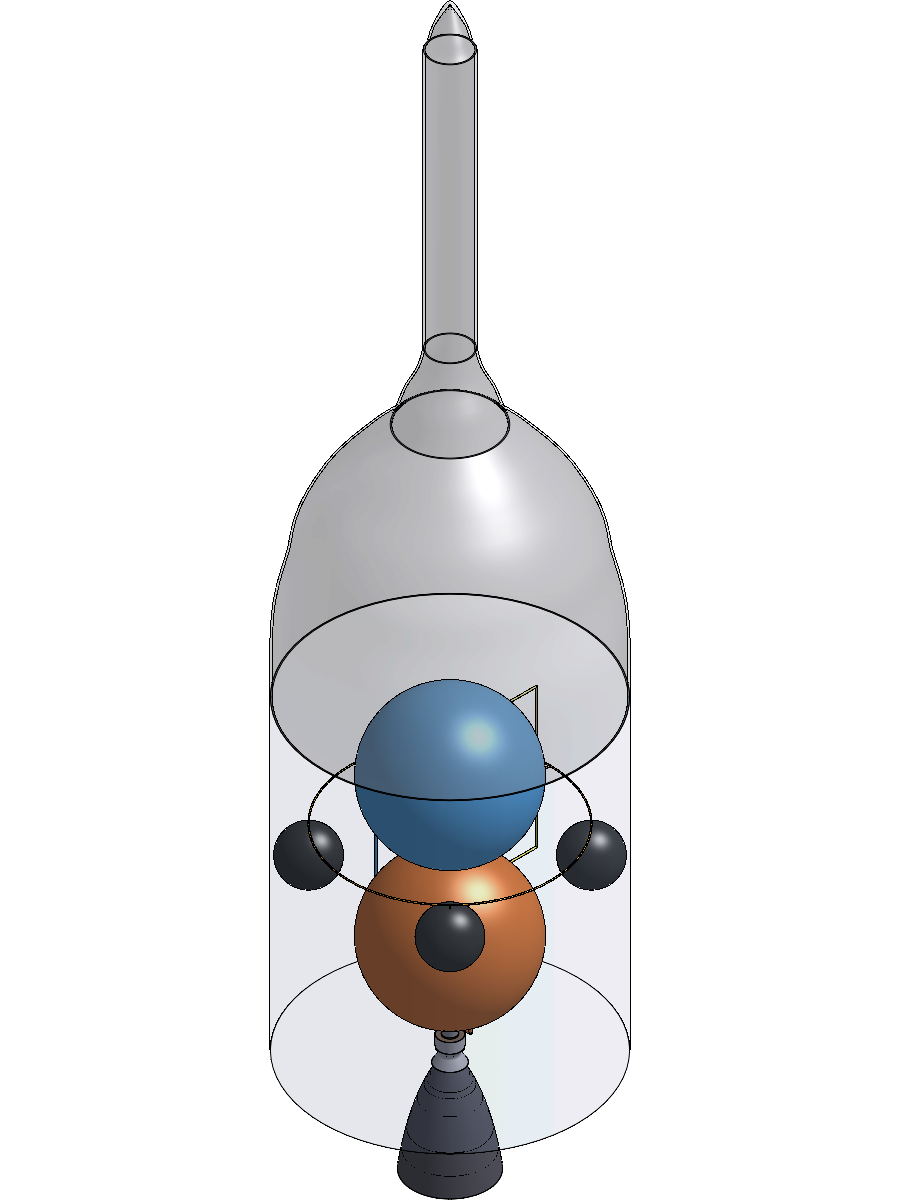
\includegraphics[width=\textwidth]{cad_iso.png}
\caption{Full model, isometric view.}\label{cad-fig:iso}\end{minipage}\hfill
\begin{minipage}{0.48\textwidth}\centering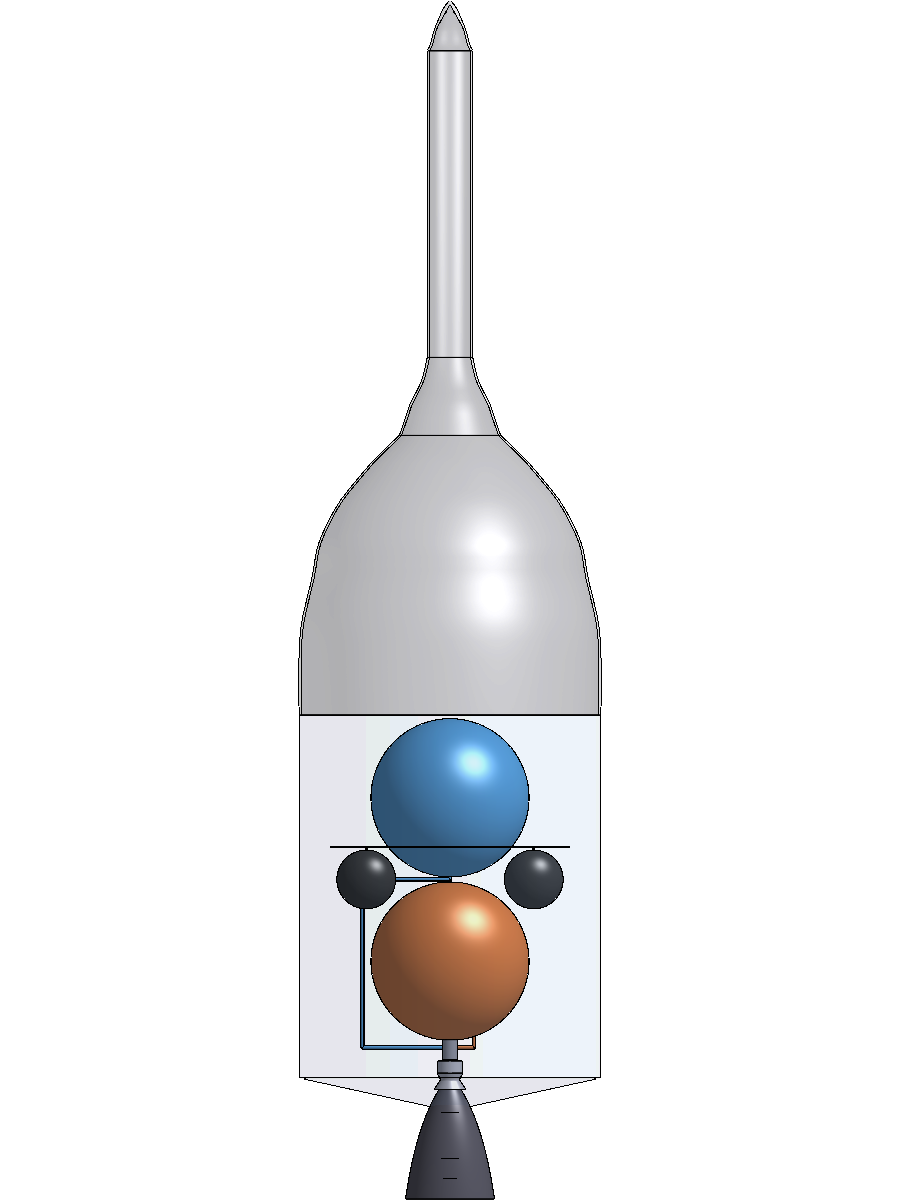
\includegraphics[width=\textwidth]{cad_front.png}
\caption{Full model, front view.}\label{cad-fig:front}\end{minipage}
\end{figure}

\subsubsection{Engine}
The ablative liner, the titanium case and the C-103 nozzle extension are each revolved 360$^\circ$ about the vehicle axis
from the analysis contour. Each is a single smooth body: the gas-side and outer contours are fitted splines through the
contour stations. The cylindrical chamber section is a straight line. The extension is the gas-side spline surface
thickened outward by a constant 0.6~mm. It is trimmed where it meets the liner end face at area ratio 6. The liner, case
and extension stay separate parts because they are different materials.

The injector is a 20~mm 304L plate at chamber diameter with twelve quarter-wave acoustic cavities, each 59.4~mm deep (Table~\ref{tab:acoustic}).
The analysis gives only the number and depth of the cavities, so they are modelled as axial \O16~mm bores on a 100~mm
pitch radius. The valve, gimbal and head stack is a cylinder 350~mm long, from the injector face to the gimbal plane. Its
density is set so that the cylinder carries the 44~kg budgeted in Table~\ref{tab:mass} for valves, gimbal actuators and miscellaneous items.

\subsubsection{Tanks, pressurant and envelope}
The NTO and MMH tanks are Ti-6Al-4V spherical shells. The helium bottles are spherical shells with a 20~mm wall and a
density chosen to carry the composite overwrapped pressure vessel (COPV) mass in Table~\ref{tab:mass}. The SM envelope (4.98~m diameter,
6~m long, 0.5~m aft cone) is a transparent reference body. The capsule and LES outer shape is a 20~mm reference shell with
no mass. It was traced from the PDR drawing [C2], scaled to the 4.98~m SM diameter and the 11.8~m height from the SM top
to the LES tip. The drawing's 0.41~m dimension lands on the LES nose. The tower, as drawn, is about 0.74~m in diameter,
and the model follows the drawing.

\subsubsection{Cut view}
The feature has a \emph{Cut view} checkbox that removes the $-Y$ half of every body. This exposes the engine section, the
hollow tanks and bottles, and the feed lines, which lie in the cut plane (Figs.~\ref{cad-fig:cutfront}--\ref{cad-fig:cutengine}).
Mass properties must be read with the cut view off. Onshape's own section-view tool gives the same picture without
changing the model.

\begin{figure}[htbp]\centering\graphicspath{{./}{figs/}{images/}{figures/}{Figures/}}
\begin{minipage}{0.48\textwidth}\centering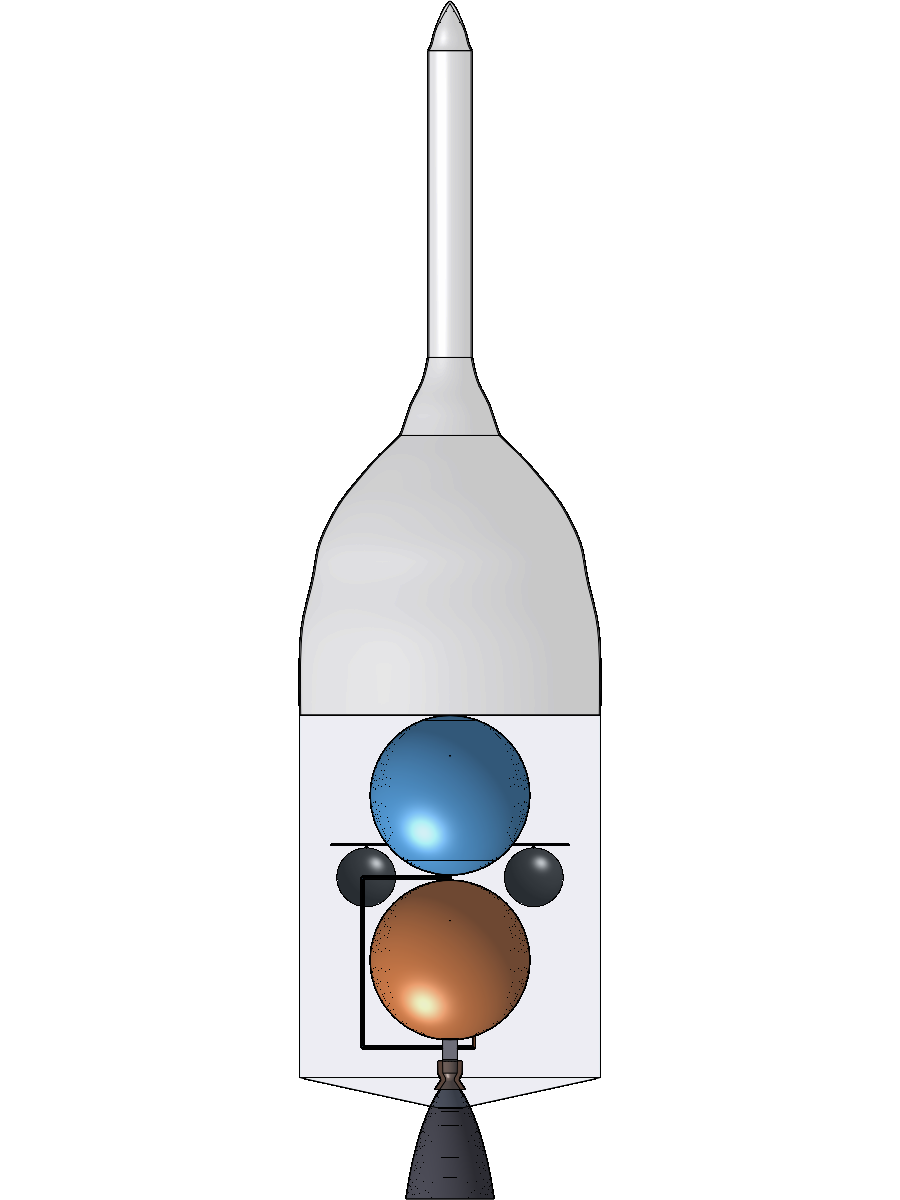
\includegraphics[width=\textwidth]{cad_cut_front.png}
\caption{Cut view, front.}\label{cad-fig:cutfront}\end{minipage}\hfill
\begin{minipage}{0.48\textwidth}\centering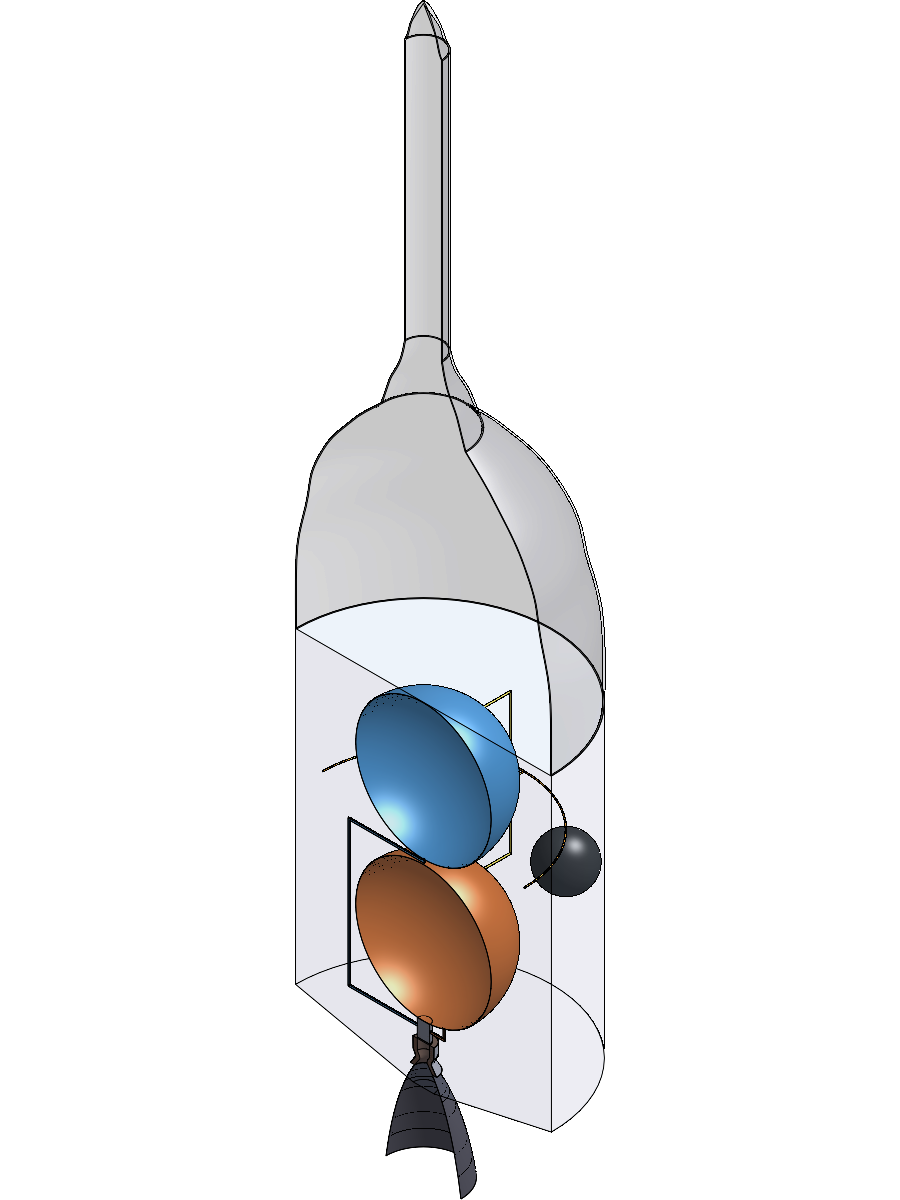
\includegraphics[width=\textwidth]{cad_cut_iso.png}
\caption{Cut view, isometric.}\label{cad-fig:cutiso}\end{minipage}
\end{figure}
\begin{figure}[htbp]\centering\graphicspath{{./}{figs/}{images/}{figures/}{Figures/}}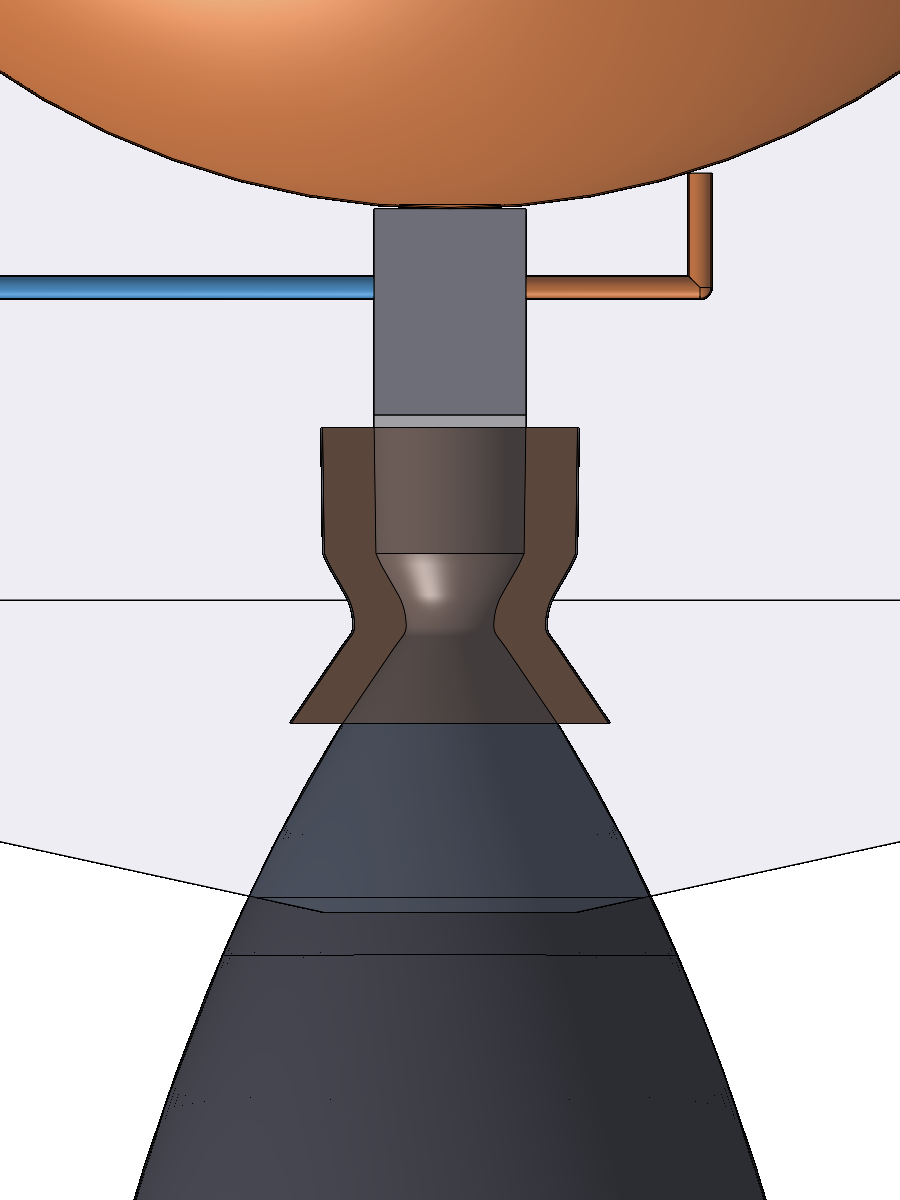
\includegraphics[width=0.6\textwidth]{cad_cut_engine.png}
\caption{Cut view of the engine: head stack, injector, silica-phenolic liner and Ti case, throat, and the start of the
C-103 extension, with the NTO (right) and MMH (left) feed lines entering the valve stack.}\label{cad-fig:cutengine}\end{figure}

\subsection{Changes from the Analysis Layout}\label{cad-sec:changes}
\begin{itemize}
\item \textbf{Tank size.} The tanks follow the PDR drawing [C2]: 2.6~m inner diameter, 9.203~m$^3$ each. The wall is
scaled from Sec.~\ref{sec:tanks} to 2.14~mm, which keeps the same maximum operating pressure and allowable stress. The two tanks are the
same size by design. At O/F~1.65, the NTO (1,440~kg/m$^3$) and MMH (875~kg/m$^3$) loads occupy 9.08 and 9.06~m$^3$
(PDR requirements 1.2.2-01/02 [C1]). Section~\ref{sec:tanks} enlarged the tanks to 2.63~m for 5~\% ullage. With 2.6~m tanks,
the free volume is only 1.3~\% (NTO) and 1.6~\% (MMH), which is below the usual 3--5~\%. This is an open item: either
return to 2.63~m or offload about 3~\% of the propellant.
\item \textbf{Tank stacking.} The analysis placed the NTO tank from its inner diameter, so its 2.16~mm wall overlapped
the head stack by 19.4~cm$^3$. Both tanks now sit on their outer surfaces. The NTO centre is at $z = 1{,}928$~mm and
the MMH centre at $z = 4{,}632$~mm, with a 100~mm gap between the tanks and 65~mm clearance to the SM top. The helium
bottles keep the same rules as before: 50~mm above the NTO tank and 50~mm from the SM wall.
\item \textbf{Lines added.} The analysis sized the feed lines but did not lay them out. The routing and the helium line
sizes are new (Sec.~\ref{cad-sec:lines}).
\end{itemize}
A two-bottle helium layout ($2\times1.206$~m COPVs, same total volume) was also checked. It fitted with 376~mm tank
clearance, but the four-bottle baseline was retained.

\subsection{Feed and Pressurization Lines}\label{cad-sec:lines}
The system is pressure-fed with regulated helium. Four 31~MPa COPVs supply a regulator that holds both tank ullages at
1.33~MPa, and the tank pressure drives the propellants to the engine (Sec.~\ref{sec:tanks}). All lines are 321 stainless steel
(Table~\ref{cad-tab:lines}). The propellant line size is taken from the feed analysis (Table~\ref{tab:lines}). The helium lines were sized
for this model:
\begin{itemize}
\item \textbf{High-pressure line.} The governing load is the 31~MPa bottle pressure. A 3/8~in~$\times$~0.065~in tube
then sees a 90~MPa hoop stress, a factor of 5.7 on ultimate.
\item \textbf{Low-pressure lines.} These are sized by the helium flow that replaces the outflowing propellant, 3.4~L/s
per tank. A 3/4~in~$\times$~0.049~in tube keeps the helium velocity near 16~m/s.
\end{itemize}

The regulator and check-valve panel is a lumped 10~kg block. Valves, filters, the flexible sections each feed line needs
where it crosses the gimbal, the propellant management devices and the line supports are not modelled.

\begin{table}[htbp]\centering\small\caption{Feed and pressurization lines.}\label{cad-tab:lines}
{\footnotesize\setbox0=\hbox{\begin{tabular}{p{0.13\linewidth}p{0.17\linewidth}p{0.24\linewidth}p{0.31\linewidth}}\hline
Line & OD $\times$ wall & Basis & Route \\\hline
NTO feed & 1.5~in $\times$ 0.065~in & 4.95~kg/s at 3.6~m/s; 64~kPa line loss & NTO lower dome ($r = 400$~mm), down, into the $+X$ side of the valve stack at $z = 500$~mm \\
MMH feed & 1.5~in $\times$ 0.065~in & 3.00~kg/s at 3.6~m/s; 50~kPa line loss & MMH bottom pole, through the tank gap, down at $x = -1{,}450$~mm outside the NTO tank, into the $-X$ side of the valve stack \\
He high pressure & 0.375~in $\times$ 0.065~in & 31~MPa; hoop stress 90~MPa (factor 5.7 on ultimate) & COPV top outlets to a ring manifold ($r = 1{,}961$~mm, $z = 3{,}819$~mm), then to the regulator \\
He low pressure & 0.75~in $\times$ 0.049~in & 1.33~MPa; about 16~m/s at 3.4~L/s per tank & Regulator ($+Y$, $r = 1{,}700$~mm) to each tank's upper dome, 60$^\circ$ from the top pole \\
\hline\end{tabular}}\ifdim\wd0>\linewidth\resizebox{\linewidth}{!}{\box0}\else\box0\fi}\end{table}

\subsection{Nozzle Extension Wall}
The C-103 extension wall is 0.6~mm thick. Internal pressure does not size it. The gas pressure is 19.9~kPa at the
attach station (area ratio 6, Mach 3.0) and 0.44~kPa at the exit. With $\sigma = p r / t$, the hoop stress is 5.7~MPa
at the attach station and 0.5~MPa at the exit, which is far below the strength of C-103 at its 1,389~K peak temperature
(1,600~K limit, Sec.~\ref{sec:cool}).

Thickness also does not affect the wall temperature. A radiation-cooled skirt runs at radiation equilibrium, so a thicker
wall only adds mass. The real sizing loads are stiffness against vibration, gimbal and handling loads, and the attach
flange. The mass budget covers these with a 25~\% allowance for stiffening rings, the flange and the coating (40.7~kg
against 32.5~kg for the bare wall, Table~\ref{tab:mass}). The CAD shows the bare wall. A taper from about 1.0~mm at the flange to 0.6~mm at
the exit, with two or three hat-section stiffening rings, would represent the hardware more fully without changing the
thermal design.

\subsection{Mass Properties}
Onshape nominal mass properties, with the cut view off, are compared with the analysis mass build-up (Table~\ref{tab:mass}) in
Table~\ref{cad-tab:cadmass}. The densities used are silica phenolic 1,750, Ti-6Al-4V 4,430, C-103 8,860, 304L 7,900 and
321 stainless 8,030~kg/m$^3$. Items marked ``lumped'' have a density chosen to match the budget. The modelled masses are
bare geometry. The analysis values also include flanges, rings, manifolds and tank fittings that are not drawn.

\begin{table}[htbp]\centering\small\caption{CAD mass properties against the analysis mass build-up.}\label{cad-tab:cadmass}
{\footnotesize\setbox0=\hbox{\begin{tabular}{p{0.23\linewidth}p{0.13\linewidth}rrp{0.25\linewidth}}\hline
Part & Material & CAD, kg & Analysis, kg & Note \\\hline
Ablative liner & silica phenolic & 66.13 & 66.38 & \\
Chamber case & Ti-6Al-4V & 6.47 & 10.03 & analysis adds 3~kg of flanges \\
Nozzle extension & C-103 & 33.23 & 40.65 & analysis: 32.5~kg bare $\times$ 1.25 \\
Injector plate & 304L & 6.94 & 10.00 & analysis includes a 2.6~kg manifold \\
Head, valve and gimbal stack & lumped & 44.00 & 44.00 & valves, actuators, miscellaneous \\
NTO tank (bare shell) & Ti-6Al-4V & 201.28 & 271.92 & 2.6~m ID; analysis value includes more than the shell \\
MMH tank (bare shell) & Ti-6Al-4V & 201.28 & 271.22 & as above \\
Helium COPVs ($\times$4) & lumped & 379.94 & 379.94 & \\
Feed lines (NTO / MMH) & 321 SS & 0.70 / 8.50 & & \\
He lines (high / low pressure) & 321 SS & 4.17 / 2.01 & & \\
Lines total & & 15.38 & 12.93 & the MMH line is 5.6~m long because it routes around the NTO tank \\
Regulator panel & lumped & 10.00 & -- & part of the 40~kg components budget \\
\hline\end{tabular}}\ifdim\wd0>\linewidth\resizebox{\linewidth}{!}{\box0}\else\box0\fi}\end{table}

\subsection{Interference Check}
Every pair of the 17 hardware bodies (136 pairs) was intersected on copies in Onshape. There is no interference. The
largest overlap of any pair is $4\times10^{-5}$~mm$^3$, which is numerical noise at tangent contacts. Connected parts
meet with gaps of 0--0.12~mm. The 0.12~mm gap is at the MMH outlet, where the flat tube end meets the curved dome.
Selected clearances:
\begin{itemize}
\item NTO to MMH tank: 95.7~mm.
\item Bottles to the SM wall: 50~mm.
\item Bottles to the propellant tanks: 601~mm.
\end{itemize}
Against the SM envelope, only the C-103 extension lies outside (3.27~L). This is expected, because the nozzle exit is
2.01~m below the SM base and the aft cone is only 0.5~m deep.

\subsection{Performance Verification with RocketCEA}\label{cad-sec:cea}
The ideal design point of Table~\ref{tab:ideal} was re-run with RocketCEA 1.2.3 [C4]: N$_2$O$_4$/MMH, $P_c = 0.862$~MPa, O/F~1.65, area
ratio 108, infinite-area combustor, with frozen flow frozen at the chamber.

RocketCEA's built-in propellant cards use different heats of formation from the NASA database used above. For example,
N$_2$O$_4$(l) is $-19.56$~kJ/mol in RocketCEA against $-17.55$~kJ/mol in the database. The comparison therefore uses
custom cards with the database values and the 293.15~K propellant temperature used above. The default cards are shown for
reference (Table~\ref{cad-tab:cea}).

\begin{table}[htbp]\centering\small\caption{Ideal vacuum performance: analysis solver against RocketCEA.}\label{cad-tab:cea}
{\footnotesize\setbox0=\hbox{\begin{tabular}{lrrrrr}\hline
 & This & RocketCEA, & & RocketCEA, & \\
Quantity & report & same basis & Diff. & default cards & Diff. \\\hline
$T_c$, K & 3{,}042.3 & 3{,}045.7 & +0.11~\% & 3{,}044.6 & +0.08~\% \\
$\mathcal{M}_c$, g/mol & 20.42 & 20.41 & $-$0.03~\% & 20.41 & $-$0.02~\% \\
$c^*$, shifting, m/s & 1{,}737.9 & 1{,}739.4 & +0.08~\% & 1{,}738.9 & +0.06~\% \\
$C_{F,vac}$, shifting & 1.9276 & 1.9281 & +0.03~\% & 1.9280 & +0.02~\% \\
$I_{sp,vac}$, shifting, s & 341.50 & 341.99 & +0.14~\% & 341.87 & +0.11~\% \\
Exit pressure, shifting, Pa & 429.9 & 430.3 & +0.09~\% & 430.2 & +0.06~\% \\
$c^*$, frozen, m/s & 1{,}698.6 & 1{,}699.8 & +0.07~\% & 1{,}699.4 & +0.05~\% \\
$C_{F,vac}$, frozen & 1.8753 & 1.8753 & 0.00~\% & 1.8753 & 0.00~\% \\
$I_{sp,vac}$, frozen, s & 324.71 & 325.04 & +0.10~\% & 324.97 & +0.08~\% \\
\hline\end{tabular}}\ifdim\wd0>\linewidth\resizebox{\linewidth}{!}{\box0}\else\box0\fi}\end{table}

Every quantity agrees within 0.3~\%, exit temperature included. This confirms the ideal performance on which the
delivered 320.8~s specific impulse is built.

\subsection{Compliance with the Mission Breakdown}\label{cad-sec:mb}
The design was checked against every value in the Crew Capsule tab of the mission breakdown spreadsheet [C3]
(Table~\ref{cad-tab:mb}). All values are met except the propellant volume at high propellant temperature. NTO expands
as it warms. In the 2.6~m PDR tanks (9.203~m$^3$), the 13,076~kg NTO load leaves 2.9~\% free volume at 10~$^\circ$C,
1.35~\% at 20~$^\circ$C and 0.56~\% at 25~$^\circ$C, and it does not fit at the 32~$^\circ$C hot case ($-0.57$~\%).
The MMH tank keeps 0.8~\% at 32~$^\circ$C. The analysis tank sizes (2.633~m MMH, 2.635~m NTO) give 3.4~\% at 32~$^\circ$C
and fit the SM if the gap between the tanks is reduced from 100 to 90~mm.

\begin{table}[htbp]\centering\small\caption{Design against the Crew Capsule mission breakdown.}\label{cad-tab:mb}
{\footnotesize\setbox0=\hbox{\begin{tabular}{p{0.19\linewidth}p{0.27\linewidth}p{0.38\linewidth}}\hline
Item & Mission breakdown & Design \\\hline
Thrust, engines & 25~kN, 1 engine & 25~kN vacuum, 1 engine (met) \\
Specific impulse & 280~s & 320.8~s delivered, 303.5~s pessimistic (met) \\
$\Delta v$ & 2,209~m/s & 2,531~m/s, 2,394~m/s pessimistic (met) \\
$M_0$, $M_p$, $M_b$ & 38,000 / 21,000 / 17,000~kg & unchanged (met) \\
$\dot m \times t_b$ & 9.10~kg/s $\times$ 2,307~s & 7.94~kg/s $\times$ 2,644~s = 21,000~kg; liner life 3,305~s (met) \\
$T/W$ at the Moon & 0.405 full, 0.905 empty & unchanged (met) \\
Structural mass $M_s$ & 6,500~kg & propulsion system 1,373~kg, 21.1~\% (met) \\
Propellant volume & 21,000~kg at O/F 1.65 & fits up to about 28~$^\circ$C in 2.6~m tanks (open item) \\
\hline\end{tabular}}\ifdim\wd0>\linewidth\resizebox{\linewidth}{!}{\box0}\else\box0\fi}\end{table}

\subsection{Conclusions}
The service-module propulsion system is modelled as one parametric Onshape feature built directly from the analysis
outputs. It includes the engine, the PDR-size tanks, four helium bottles, sized feed and pressurization lines, and
reference shells for the SM, the capsule and the LES. The model has no interferences, and its masses agree with the
analysis budget once the undrawn flanges, rings and fittings are accounted for. The 0.6~mm C-103 extension wall is
adequate for pressure and temperature; its sizing loads are stiffness and handling, which are covered by the ring
allowance. RocketCEA reproduces the analysis performance within 0.3~\%. Two items remain open: the 1.3--1.6~\% ullage of
the 2.6~m PDR tanks, and the flex sections the feed lines need across the gimbal.

\subsection*{References for this section}
{\small\begin{description}
\item[{[C1]}] Kempf, A., Bratt, E., LeRoy, M., Bernal, R., Wiser, S., and Rouland, S., ``Project ABEONA Preliminary Design Report,'' unpublished class report, 2026.
\item[{[C2]}] Kempf, A., Bratt, E., LeRoy, M., Bernal, R., Wiser, S., and Rouland, S., ``Preliminary Design Review, Project ABEONA,'' unpublished class presentation, slide 7 (Crew Capsule), 2026.
\item[{[C3]}] Project ABEONA, \texttt{Mission\_Breakdown.xlsx}, Crew Capsule tab, 2026.
\item[{[C4]}] Taylor, C., ``RocketCEA,'' Python wrapper for NASA CEA, version 1.2.3, rocketcea.readthedocs.io.
\item[{[C5]}] Gordon, S. and McBride, B. J., ``Computer Program for Calculation of Complex Chemical Equilibrium Compositions and Applications,'' NASA RP-1311, 1994.
\end{description}}

\section{Conclusions}
A pressure-fed NTO/MMH engine was designed for the Crew Capsule. At 0.862~MPa chamber pressure, O/F 1.65 and area ratio
\NEPS, it delivers 25~kN at \NIspD~s vacuum $I_{sp}$ (\NIspP~s pessimistic), meeting the 280~s requirement. The 80~\% Rao bell
(\NDe~m exit) is optimized for vacuum and fits the \NLavail~m length available. The silica-phenolic chamber, protected
by a fuel-rich outer ring, survives \Ntdesign~s without throat wear, and the C-103 extension stays below \NTmaxExt~K. The
two titanium tanks and four helium bottles fit the PDR service-module section.

Open risks: the heat flux and the fuel-rich ring have not been calibrated by test; the ablator properties are assumed;
the injector soak-back depends on the insulating ring; and the titanium tanks require controlled NTO.

\begin{thebibliography}{99}\small
\bibitem{hh} Huzel, D. K. and Huang, D. H., \emph{Modern Engineering for Design of Liquid-Propellant Rocket Engines}, AIAA Progress in Astronautics and Aeronautics Vol. 147, 1992 (Eq. 4-13; Eq. 4-36; Table 4-1; Ch. 5; Sec. 4.4).
\bibitem{cea} Gordon, S. and McBride, B. J., \emph{Computer Program for Calculation of Complex Chemical Equilibrium Compositions and Applications}, NASA RP-1311, 1994.
\bibitem{sb} Sutton, G. P. and Biblarz, O., \emph{Rocket Propulsion Elements}, 9th ed., Wiley, 2017 (Ch. 3, Ch. 8).
\bibitem{sp} NASA SP-8089 \emph{Liquid Rocket Engine Injectors} (1976); SP-8112 \emph{Pressurization Systems for Liquid Rockets} (1975); SP-8088 \emph{Liquid Rocket Metal Tanks and Tank Components} (1974).
\bibitem{rcea} Taylor, C., \emph{RocketCEA documentation}, N2O4/MMH performance table and kinetic-peak mixture-ratio charts, \url{https://rocketcea.readthedocs.io}.
\bibitem{rp} Taylor, C., \emph{RocketProps}, \url{https://rocketprops.readthedocs.io}.
\bibitem{and} Anderson, J. D., \emph{Modern Compressible Flow}, 3rd ed., McGraw-Hill, 2003 (Ch. 11).
\bibitem{zh} Zucrow, M. J. and Hoffman, J. D., \emph{Gas Dynamics}, Vol. 2, Wiley, 1977.
\bibitem{bartz} Bartz, D. R., ``A Simple Equation for Rapid Estimation of Rocket Nozzle Convective Heat Transfer Coefficients,'' \emph{Jet Propulsion}, Vol. 27, No. 1, 1957, pp. 49--51.
\bibitem{rao} Rao, G. V. R., ``Exhaust Nozzle Contour for Optimum Thrust,'' \emph{Jet Propulsion}, Vol. 28, No. 6, 1958, pp. 377--382.
\bibitem{nasacea} NASA Glenn, CEA thermodynamic database \texttt{thermo.inp}, \url{https://github.com/nasa/cea}.
\bibitem{abeona} Project ABEONA, \texttt{Mission\_Breakdown.xlsx} and \emph{Preliminary Design Report}, Embry-Riddle Aeronautical University, 2026.
\bibitem{ethan} Bratt, E., ``Project ABEONA Stage 2 / Stage 3 Hydrolox Engine: Thrust Chamber, Cycle, and Feed System Design,'' Rev. 1, October 2026.
\bibitem{esa} ESA, ``European Service Module Propulsion,'' \url{https://www.esa.int/Science_Exploration/Human_and_Robotic_Exploration/Orion/European_Service_Module_Propulsion}.
\bibitem{belair} Belair, M. et al., ``Artemis I Engine Performance,'' NTRS 20240003648, 2024 (pp. 3, 6).
\bibitem{bert} Bertolino, J. D. and Boyd, W. C., ``Uprated OMS Engine Status -- Sea Level Testing Results,'' NTRS 19910014943, 1990 (pp. 241--249).
\end{thebibliography}
\end{document}
